\documentclass{slide}
\usepackage{tikz}

\usetikzlibrary{arrows}

\usepackage{tabto}

\usepackage{languages}

% \usepackage{pgfpages}
% \setbeameroption{show notes on second screen}

\title{Distributed Computing II}
\subtitle{CSSE6400}
\author{Brae Webb}
\date{\week{6}}

% \titlegraphic {
%     \tweet%
%     {images/mathiasverraes}%
%     {Mathias Verras}%
%     {mathiasverraes}%
%     {There are only two hard problems in distributed systems:  2. Exactly-once delivery 1. Guaranteed order of messages 2. Exactly-once delivery}%
%     {https://twitter.com/mathiasverraes/status/632260618599403520}%
% }

\begin{document}

\maketitle

\point[Previously in CSSE6400\dots]{
\begin{center}
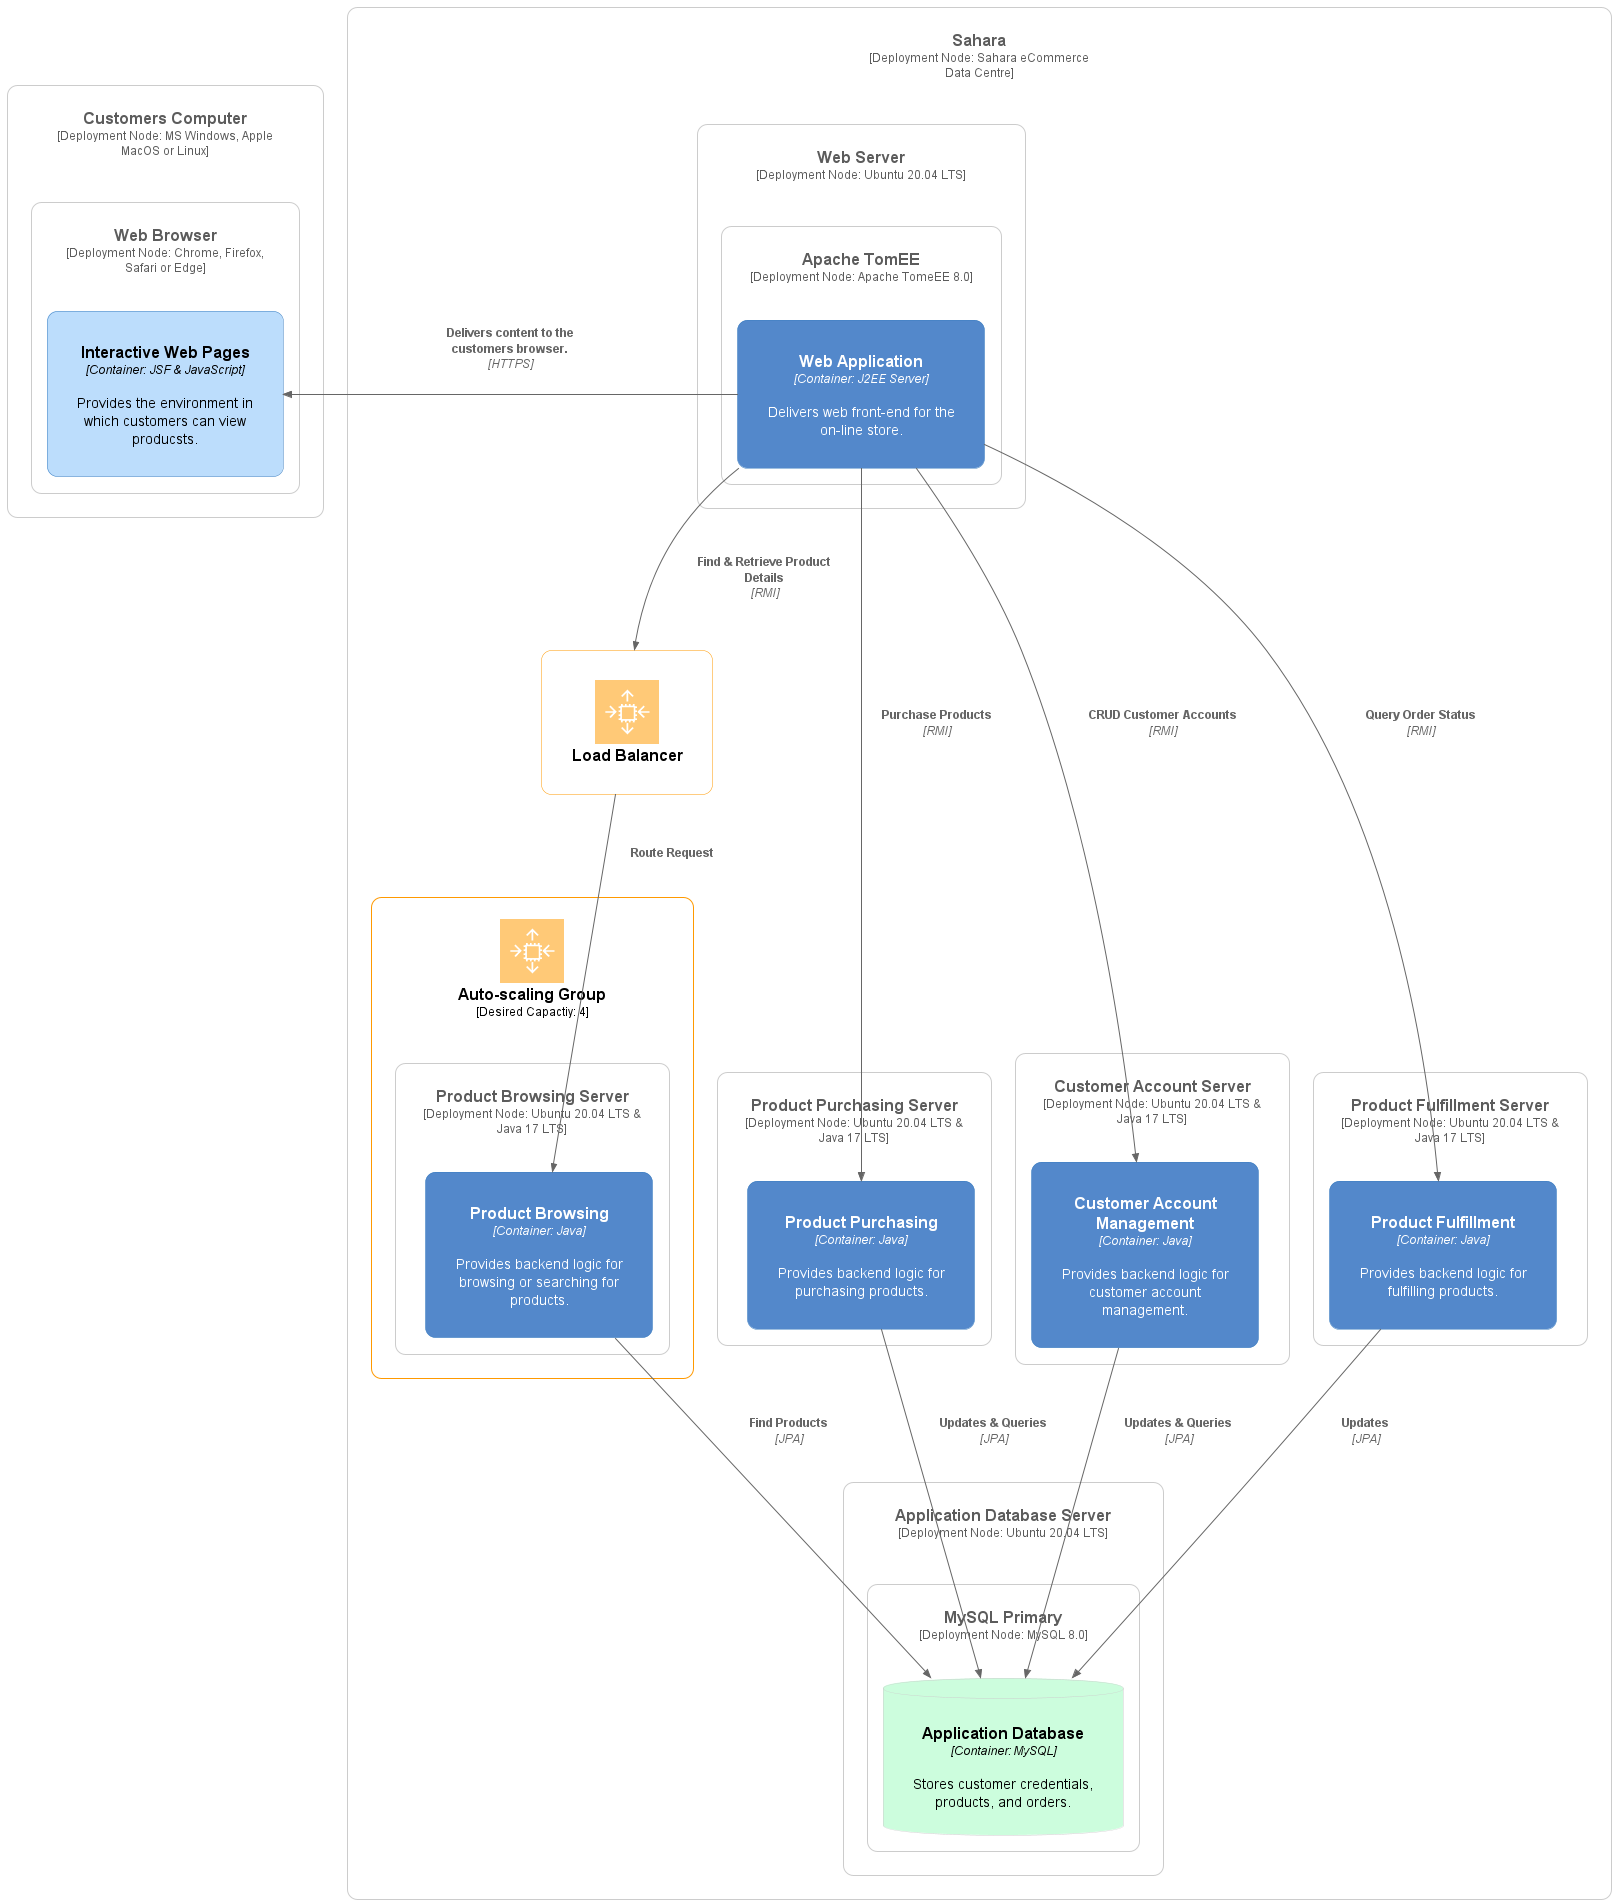
\includegraphics[width=0.8\textheight]{diagrams/SaharaScaled}
\end{center}
}

\point[Things start going wrong]{What is the likely cause?}

\point[Database]{
\begin{center}
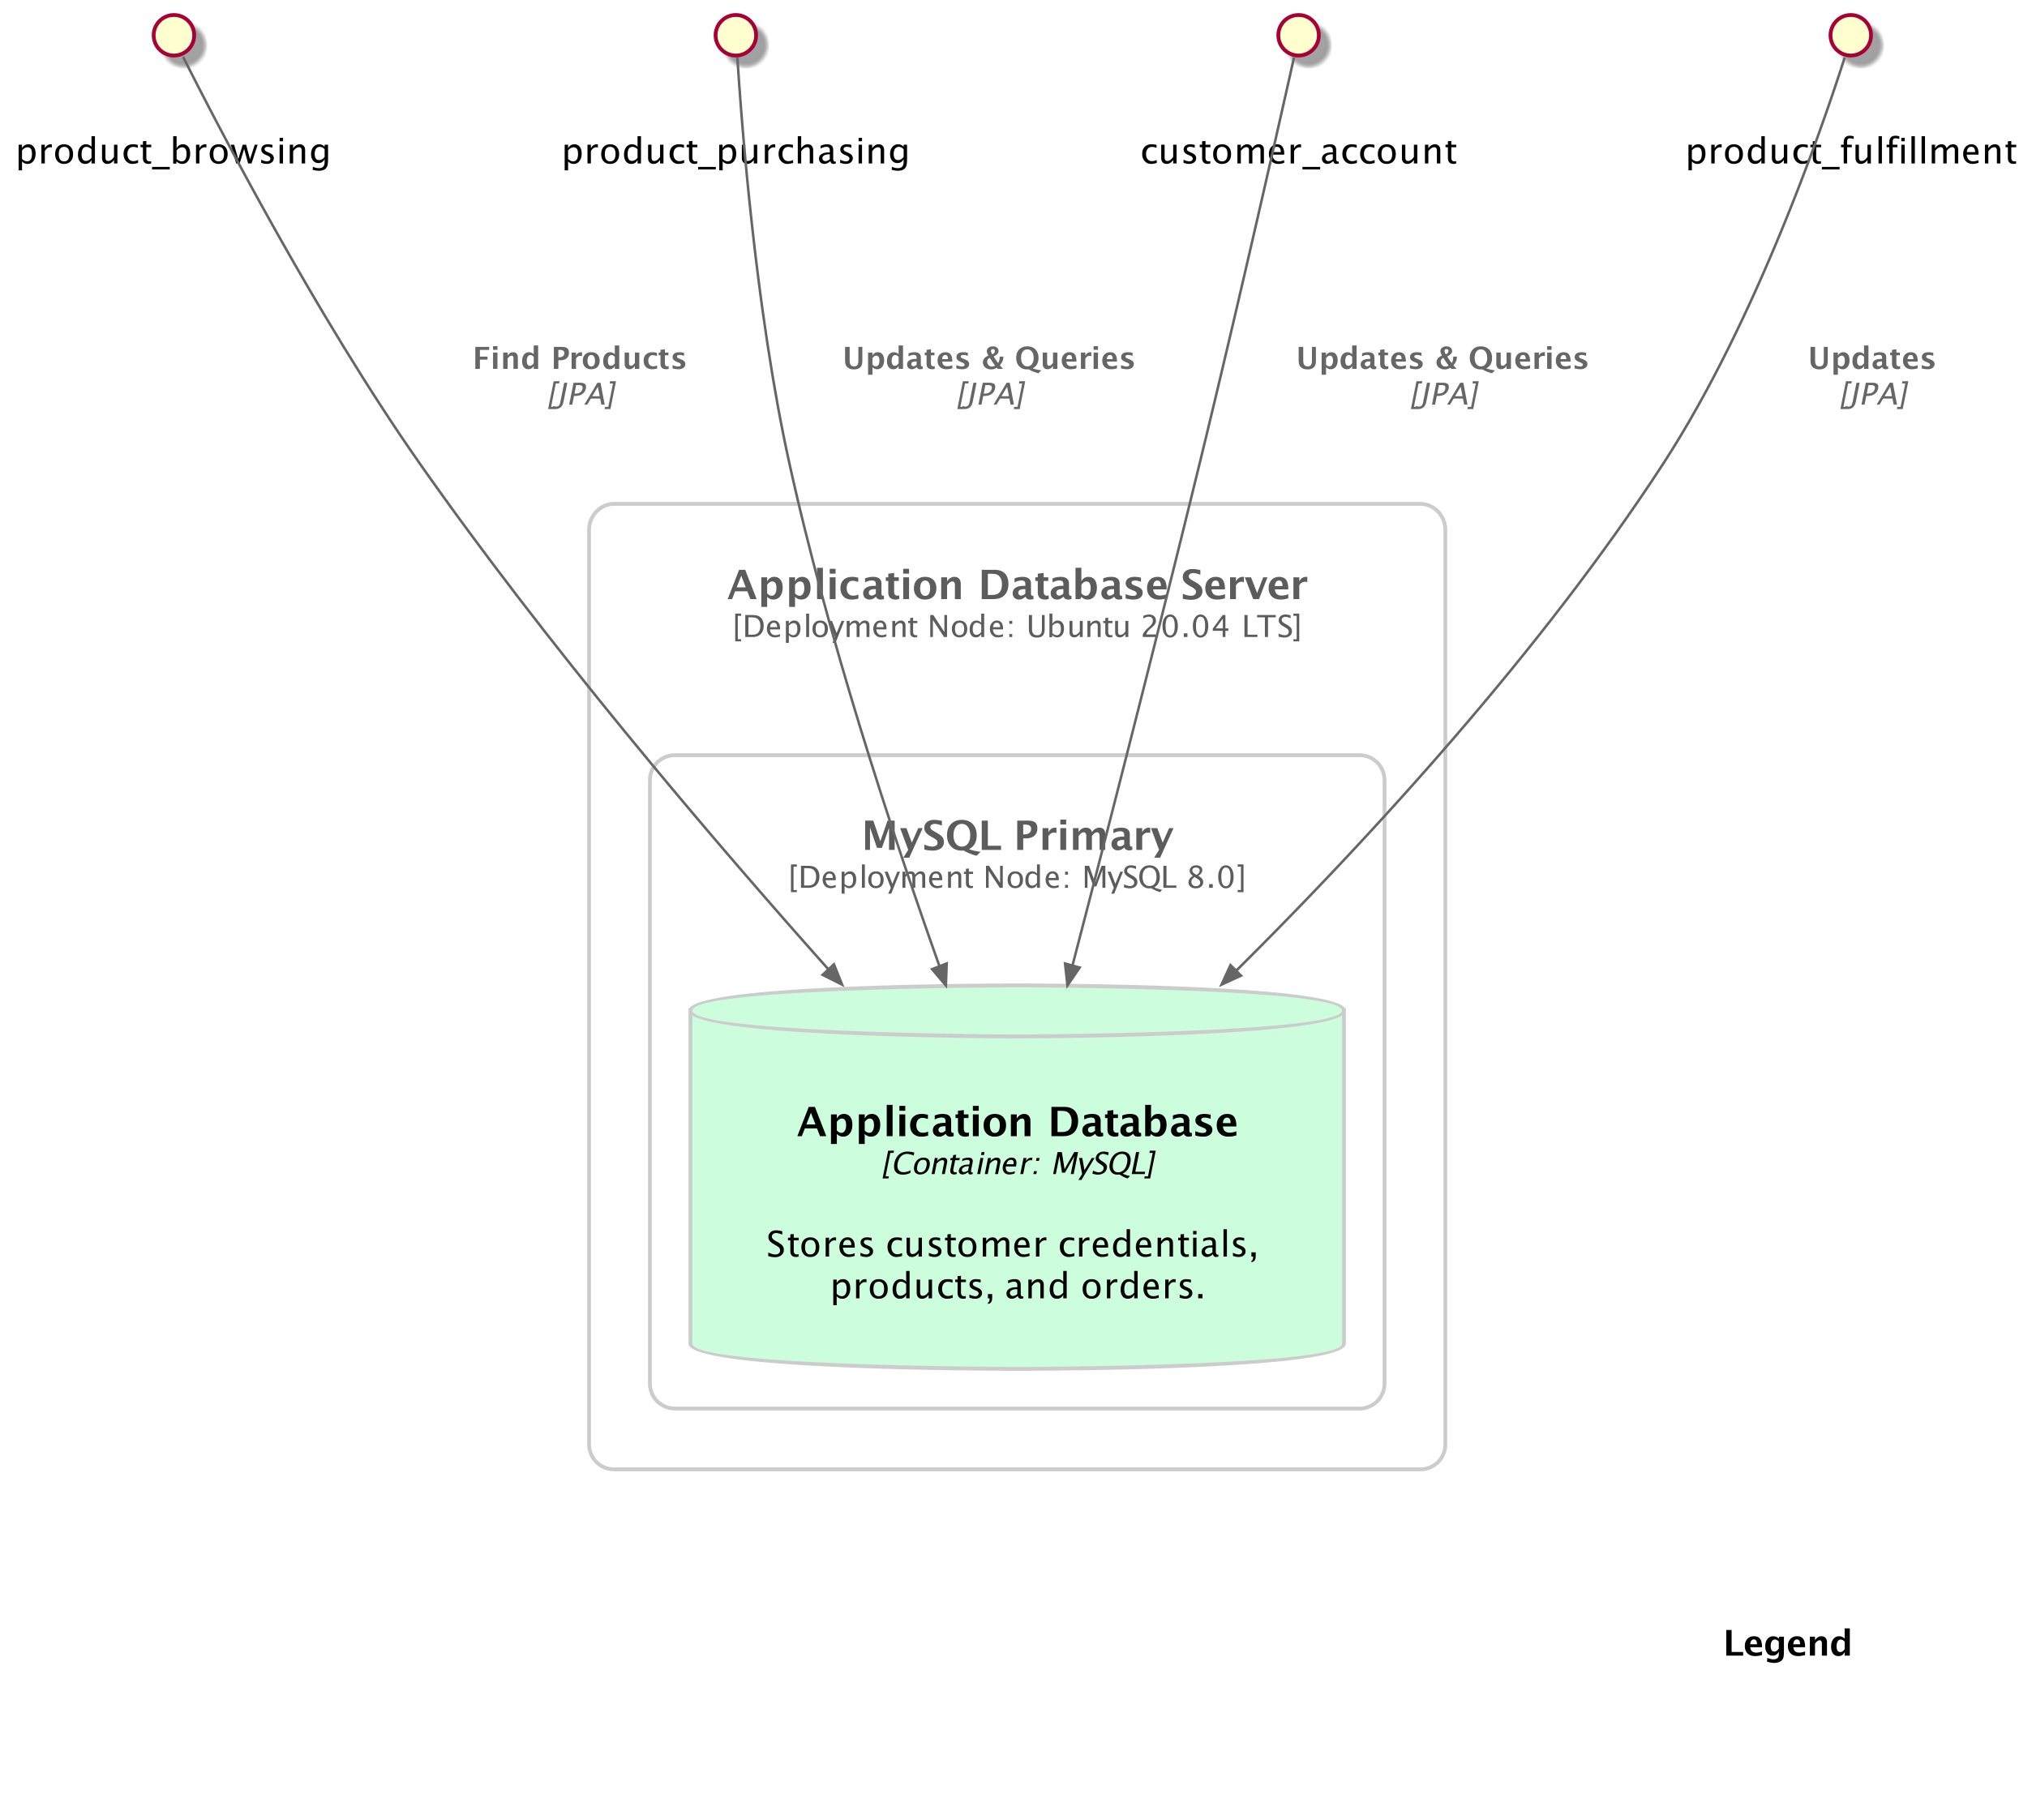
\includegraphics[width=\textheight]{diagrams/FocusDB}
\end{center}
}


%%%%%%%%%%%%%%%
% Replication %
%%%%%%%%%%%%%%%
\questionanswer{How do we fix database scaling issues?}{
    \begin{itemize}
        \item
        \only<3->{\highlight{Replication}}
        \only<-2>{Replication}
        \item Partitioning (or sharding)
        \item Independent databases
    \end{itemize}
}

\question{What is \highlight{replication}?}

\definition{Replication}{
    Data copied across multiple different machines.
}

\definition{Replica}{
    Database node which stores a copy of the data.
}


\questionanswer{What are the advantages of \highlight{replication}?}{
    \begin{itemize}[<+(1)->]
        \item Scale out our database to cope with load.
        \item Provide fault tolerance from a single database instance failure.
        \item Locate databases closer to end-users.
    \end{itemize}
}

\image{diagrams/LeaderFollower}

\point[Leader-based Replication]{
    \begin{description}[<+->]
        \item[On write] Writes sent to leader, change is propagated via change stream.
        \item[On read] Any replica can be queried. 
    \end{description}
}

\image{diagrams/LeaderFollowerSpread}

\point[Propogating changes]{
    \highlight{Synchronous} vs. \highlight{Asynchronous}
}

\point[When things go wrong]{
    Handling outages
}

\point{Follower failure}

\point{Leader failure}

%%%%%%%%%%%%%%%%
% Partitioning %
%%%%%%%%%%%%%%%%
\questionanswer{How do we fix database scaling issues?}{
    \begin{itemize}
        \item 
        \only<-2>{\highlight{Replication}}
        \only<3->{Replication}
        \item 
        \only<3->{\highlight{Partitioning (or sharding)}}
        \only<-2>{Partitioning (or sharding)}
        \item Independent databases
    \end{itemize}
}


%%%%%%%%%%%%%%%%%%%%%%%%%%%%%
% Isolation (foreshadowing) %
%%%%%%%%%%%%%%%%%%%%%%%%%%%%%
\questionanswer{How do we fix database scaling issues?}{
    \begin{itemize}
        \item Replication
        \item 
        \only<-2>{\highlight{Partitioning (or sharding)}}
        \only<3->{Partitioning (or sharding)}
        \item 
        \only<3->{\highlight{Independent databases}}
        \only<-2>{Independent databases}
    \end{itemize}
}

% \references{articles,books}

\end{document}